% ==============================================================================
% =================================== Aufgabe 2 ================================
% ==============================================================================

\chapter{Aufgabe (2)}
\label{chap:Aufgabe2}
\thispagestyle{fancy}

Die folgende Aufgabe basiert auf dem \texttt{California Housing}-Datensatz, der in der Bibliothek \texttt{sklearn.datasets} enthalten ist. Der Datensatz enthält Informationen über Häuser in verschiedenen Distrikten Kaliforniens und wird für Regressionsaufgaben verwendet.

% ======================================= a =====================================

\section{Bibliotheken importieren, Datensatz laden und beschreiben (a)}
\label{sec:2a}

\subsection{Aufgabenstellung}

Die erforderlichen Bibliotheken werden importiert, der \texttt{California Housing}-Datensatz wird geladen und eine Beschreibung des Datensatzes wird ausgegeben. Die Attribute des Datensatzes werden kurz beschrieben.

\subsection{Lösung}

Zunächst werden die benötigten Bibliotheken importiert: \texttt{sklearn.datasets} zum Laden des Datensatzes, \texttt{pandas} für die spätere Datenverarbeitung sowie \texttt{matplotlib} und \texttt{seaborn} für die Visualisierung. Der Datensatz wird mit der Funktion \\ \texttt{fetch\_california\_housing()} geladen. Die Beschreibung des Datensatzes wird mit \texttt{california.DESCR} ausgegeben.

\lstinputlisting[
    language=Python, 
    caption={Bibliotheken importieren, Datensatz laden und beschreiben}, 
    label={lst:aufgabe2a}
]{asset/code/Aufgabe2a.tex}

\subsection{Ausgabe}

Die Ausgabe zeigt die Beschreibung des \texttt{California Housing}-Datensatzes:

\begin{verbatim}
.. _california_housing_dataset:

California Housing dataset
--------------------------

**Data Set Characteristics:**

:Number of Instances: 20640

:Number of Attributes: 8 numeric, predictive attributes and the target

:Attribute Information:
    - MedInc        median income in block group
    - HouseAge      median house age in block group
    - AveRooms      average number of rooms per household
    - AveBedrms     average number of bedrooms per household
    - Population    block group population
    - AveOccup      average number of household members
    - Latitude      block group latitude
    - Longitude     block group longitude

:Missing Attribute Values: None

This dataset was obtained from the StatLib:
https://lib.stat.cmu.edu/datasets/houses.zip

The target variable is the median house value for California districts,
expressed in hundreds of thousands of dollars ($100,000).

This dataset was derived from the 1990 U.S. census, using one row per census
block group. A block group is the smallest geographical unit for which the U.S.
Census Bureau publishes sample data (a block group typically has a population
of 600 to 3,000 people).

A household is a group of people residing within a home. Since the average
number of rooms and bedrooms in this dataset are provided per household, these
columns may take surprisingly large values for block groups with few households
and many empty houses, such as vacation resorts.

It can be downloaded/loaded using the
:func:`sklearn.datasets.fetch_california_housing` function.

.. rubric:: References

- Pace, R. Kelley and Ronald Barry, Sparse Spatial Autoregressions,
  Statistics and Probability Letters, 33:291-297, 1997.


Feature names: ['MedInc', 'HouseAge', 'AveRooms', 'AveBedrms', 'Population', 'AveOccup', 'Latitude', 'Longitude']
Target name: ['MedHouseVal']
Data shape: (20640, 8)
\end{verbatim}

\subsection{Interpretation}

Der \texttt{California Housing}-Datensatz enthält 20.640 Instanzen und 8 numerische Attribute. Die Attribute beschreiben verschiedene Merkmale der Distrikte:

\begin{itemize}
    \item \texttt{MedInc}: Das mittlere Einkommen im Block-Gebiet.
    \item \texttt{HouseAge}: Das mittlere Alter der Häuser im Block-Gebiet.
    \item \texttt{AveRooms}: Die durchschnittliche Anzahl der Räume pro Haushalt.
    \item \texttt{AveBedrms}: Die durchschnittliche Anzahl der Schlafzimmer pro Haushalt.
    \item \texttt{Population}: Die Bevölkerungszahl des Block-Gebiets.
    \item \texttt{AveOccup}: Die durchschnittliche Anzahl der Haushaltsmitglieder.
    \item \texttt{Latitude}: Die geografische Breite des Block-Gebiets.
    \item \texttt{Longitude}: Die geografische Länge des Block-Gebiets.
\end{itemize}

Die Zielvariable ist \texttt{MedHouseVal}, der mittlere Hauswert in \texttt{\$100.000}. Es sind keine fehlenden Werte vorhanden. Der Datensatz basiert auf der \acs{US}-Volkszählung von 1990 und enthält eine Zeile pro Block-Gebiet. Ein Block-Gebiet ist die kleinste geografische Einheit, für die die \acs{US}-Volkszählungsbehörde Stichprobendaten veröffentlicht. Die Attribute \texttt{AveRooms} und \texttt{AveBedrms} können ungewöhnlich große Werte annehmen, wenn Block-Gebiete wenige Haushalte aber viele leerstehende Häuser enthalten.

\cleardoublepage

% ======================================= b =====================================

\section{Konvertieren in einen Pandas-DataFrame (b)}
\label{sec:2b}

\subsection{Aufgabenstellung}

Der geladene Datensatz wird in einen \texttt{Pandas DataFrame} konvertiert, um die weitere Verarbeitung und Analyse zu erleichtern.

\subsection{Lösung}

Der Datensatz wird mit der Funktion \texttt{pd.DataFrame()} in einen \texttt{Pandas DataFrame} konvertiert. Die Spaltennamen werden aus \texttt{california.feature\_names} übernommen. Die Zielvariable \texttt{MedHouseVal} wird als separate Spalte hinzugefügt.

\lstinputlisting[
    language=Python, 
    caption={Konvertieren in einen \texttt{Pandas DataFrame}}, 
    label={lst:aufgabe2b}
]{asset/code/Aufgabe2b.tex}

\subsection{Ausgabe}

Die Ausgabe zeigt die ersten fünf Zeilen des DataFrames:

\begin{verbatim}
Erste 5 Zeilen des DataFrames:
   MedInc  HouseAge  AveRooms  AveBedrms  Population  AveOccup  Latitude  \
0  8.3252      41.0  6.984127   1.023810       322.0  2.555556     37.88   
1  8.3014      21.0  6.238137   0.971880      2401.0  2.109842     37.86   
2  7.2574      52.0  8.288136   1.073446       496.0  2.802260     37.85   
3  5.6431      52.0  5.817352   1.073059       558.0  2.547945     37.85   
4  3.8462      52.0  6.281853   1.081081       565.0  2.181467     37.85   

   Longitude  MedHouseVal  
0    -122.23        4.526  
1    -122.22        3.585  
2    -122.24        3.521  
3    -122.25        3.413  
4    -122.25        3.422  

Informationen zum DataFrame:
<class 'pandas.DataFrame'>
RangeIndex: 20640 entries, 0 to 20639
Data columns (total 9 columns):
 #   Column       Non-Null Count  Dtype  
---  ------       --------------  -----  
 0   MedInc       20640 non-null  float64
 1   HouseAge     20640 non-null  float64
 2   AveRooms     20640 non-null  float64
 3   AveBedrms    20640 non-null  float64
 4   Population   20640 non-null  float64
 5   AveOccup     20640 non-null  float64
 6   Latitude     20640 non-null  float64
 7   Longitude    20640 non-null  float64
 8   MedHouseVal  20640 non-null  float64
dtypes: float64(9)
memory usage: 1.4 MB
None
\end{verbatim}

\subsection{Interpretation}

Der Datensatz wird mit \texttt{pd.DataFrame(\textit{california.data, \\columns=california.feature\_names})} in einen \texttt{Pandas DataFrame} konvertiert. Die Zielvariable \texttt{MedHouseVal} wird mit \texttt{california.target} als neue Spalte hinzugefügt. Die Methode \texttt{head()} gibt die ersten fünf Zeilen zurück, um die Struktur des DataFrames zu überprüfen. Die Methode \texttt{info()} zeigt die Datentypen und die Anzahl der nicht-\texttt{NULL}-Werte an, was eine erste Einschätzung der Datenqualität ermöglicht.

\cleardoublepage

% ======================================= c =====================================

\section{Summenstatistik und Mittelwert der Spalte HouseAge (c)}
\label{sec:2c}

\subsection{Aufgabenstellung}

Es wird eine Summenstatistik des Datensatzes angezeigt. Der Mittelwert der Spalte \texttt{HouseAge} wird ermittelt.

\subsection{Lösung}

Die Summenstatistik wird mit der Methode \texttt{describe()} auf dem DataFrame berechnet. Der Mittelwert der Spalte \texttt{HouseAge} wird mit \texttt{df\_california['HouseAge'].mean()} berechnet.

\lstinputlisting[
    language=Python, 
    caption={Summenstatistik und Mittelwert der Spalte \texttt{HouseAge}}, 
    label={lst:aufgabe2c}
]{asset/code/Aufgabe2c.tex}

\subsection{Ausgabe}

Die Ausgabe zeigt die Summenstatistik des Datensatzes sowie den Mittelwert der Spalte \texttt{HouseAge}:

\begin{verbatim}
Summenstatistik des Datensatzes:
             MedInc      HouseAge      AveRooms     AveBedrms    Population  \
count  20640.000000  20640.000000  20640.000000  20640.000000  20640.000000   
mean       3.870671     28.639486      5.429000      1.096675   1425.476744   
std        1.899822     12.585558      2.474173      0.473911   1132.462122   
min        0.499900      1.000000      0.846154      0.333333      3.000000   
25%        2.563400     18.000000      4.440716      1.006079    787.000000   
50%        3.534800     29.000000      5.229129      1.048780   1166.000000   
75%        4.743250     37.000000      6.052381      1.099526   1725.000000   
max       15.000100     52.000000    141.909091     34.066667  35682.000000   

           AveOccup      Latitude     Longitude   MedHouseVal  
count  20640.000000  20640.000000  20640.000000  20640.000000  
mean       3.070655     35.631861   -119.569704      2.068558  
std       10.386050      2.135952      2.003532      1.153956  
min        0.692308     32.540000   -124.350000      0.149990  
25%        2.429741     33.930000   -121.800000      1.196000  
50%        2.818116     34.260000   -118.490000      1.797000  
75%        3.282261     37.710000   -118.010000      2.647250  
max     1243.333333     41.950000   -114.310000      5.000010  

Mittelwert der Spalte HouseAge: 28.639486
\end{verbatim}

\subsection{Interpretation}

Die Summenstatistik mit \texttt{describe()} zeigt für jede numerische Spalte die wichtigsten statistischen Kennzahlen: Anzahl, Mittelwert, Standardabweichung, Minimum, 25\%-Quantil, Median (\textit{50\%}), 75\%-Quantil und Maximum. Der Mittelwert der Spalte \texttt{HouseAge} beträgt 28.64 Jahre. Dies zeigt, dass die Häuser in den Block-Gebieten im Durchschnitt etwa 29 Jahre alt sind. Die Spalte \texttt{MedHouseVal} hat einen Mittelwert von 2.07, was einem mittleren Hauswert von etwa \texttt{\$207.000} entspricht.

\cleardoublepage

% ======================================= d =====================================

\section{Pairplot des California-Housing-Datensatzes (d)}
\label{sec:2d}

\subsection{Aufgabenstellung}

Es wird ein Pairplot des California-Housing-Datensatzes erstellt. Die Bibliothek \texttt{seaborn} wird dafür importiert. Es wird analysiert, ob lineare Zusammenhänge zwischen den unabhängigen Variablen bzw. zwischen den unabhängigen Variablen und der Zielvariable erkennbar sind.

\subsection{Lösung}

Der Pairplot wird mit der Funktion \texttt{sns.pairplot()} erstellt. Die Zielvariable \texttt{MedHouseVal} wird als \texttt{hue} übergeben, um die Datenpunkte entsprechend ihrer Hauswerte einzufärben. Die Diagonalen zeigen die Verteilung jeder Variable als Histogramm. Die Plot-Größe wird mit dem Parameter \texttt{height} angepasst, um eine gute Lesbarkeit zu gewährleisten.

\lstinputlisting[
    language=Python, 
    caption={Pairplot des California-Housing-Datensatzes}, 
    label={lst:aufgabe2d}
]{asset/code/Aufgabe2d.tex}

\subsection{Ausgabe}

Die Ausgabe zeigt den Pairplot des California-Housing-Datensatzes:

\begin{figure}[h]
    \centering
    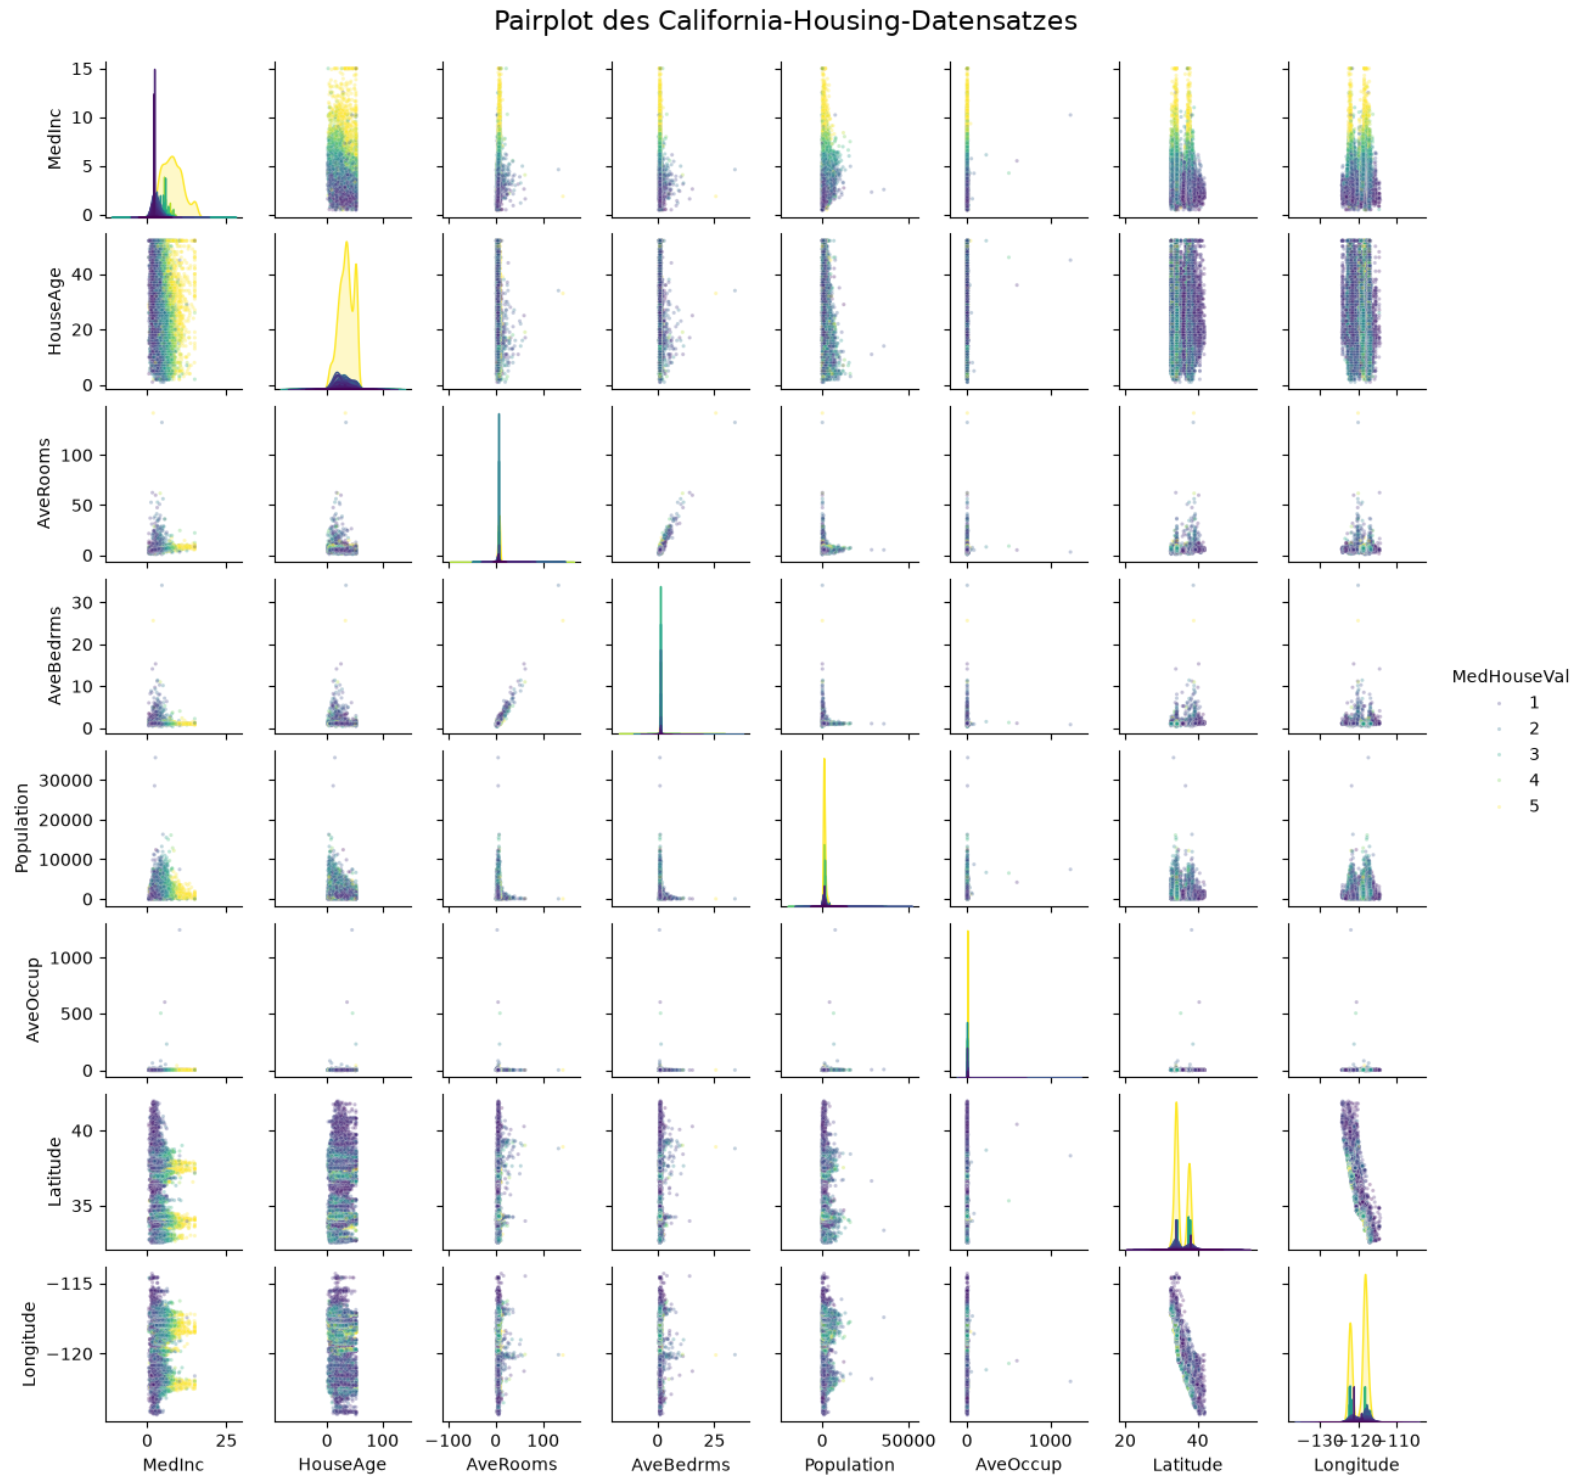
\includegraphics[width=0.9\textwidth]{./asset/image/Aufgabe2d.png}
    \caption{Pairplot des California-Housing-Datensatzes (\textit{Quelle: Eigene Darstellung})}
    \label{fig:aufgabe2d}
\end{figure}

\subsection{Interpretation}

Der Pairplot visualisiert die Beziehungen zwischen allen Attributen des Datensatzes. Auf der Diagonalen sind die Verteilungen der einzelnen Variablen als Histogramme dargestellt. Die übrigen Plots zeigen die paarweisen Beziehungen zwischen den Variablen als Scatter-Plots.

Lineare Zusammenhänge sind erkennbar zwischen:

\begin{itemize}
    \item \texttt{MedInc} und \texttt{MedHouseVal}: Es ist ein positiver, annähernd linearer Zusammenhang erkennbar. Höheres Einkommen korreliert mit höheren Hauswerten.
    \item \texttt{Latitude}/\texttt{Longitude} und \texttt{MedHouseVal}: Hier sind keine linearen Zusammenhänge erkennbar, da es sich um geografische Koordinaten handelt.
    \item \texttt{AveRooms} und \texttt{MedHouseVal}: Ein schwacher positiver Zusammenhang ist erkennbar.
    \item \texttt{Population} und \texttt{MedHouseVal}: Kein klarer linearer Zusammenhang erkennbar.
\end{itemize}

Die farbliche Kodierung der Punkte nach Hauswert (\textit{\texttt{MedHouseVal}}) zeigt, dass höhere Hauswerte in bestimmten Bereichen der geografischen Koordinaten konzentriert sind. Dies deutet auf räumliche Cluster hin, die durch die Variablen \texttt{Latitude} und \texttt{Longitude} erfasst werden.

\cleardoublepage

% ======================================= e =====================================

\section{Korrelationsplot (e)}
\label{sec:2e}

\subsection{Aufgabenstellung}

Es wird ein Korrelationsplot des California-Housing-Datensatzes erstellt. Es wird ermittelt, welche unabhängige Variable die größte Korrelation mit der Zielvariable \texttt{MedHouseVal} aufweist.

\subsection{Lösung}

Die Korrelationsmatrix wird mit der Methode \texttt{corr()} auf dem DataFrame berechnet. Der Korrelationsplot wird mit \texttt{sns.heatmap()} visualisiert. Die Korrelationen mit der Zielvariable werden extrahiert und absteigend sortiert, um die Variable mit der größten Korrelation zu identifizieren.

\lstinputlisting[
    language=Python, 
    caption={Korrelationsplot des California-Housing-Datensatzes}, 
    label={lst:aufgabe2e}
]{asset/code/Aufgabe2e.tex}

\subsection{Ausgabe}

Die Ausgabe zeigt den Korrelationsplot sowie die Korrelationen mit der Zielvariable:

\begin{figure}[h]
    \centering
    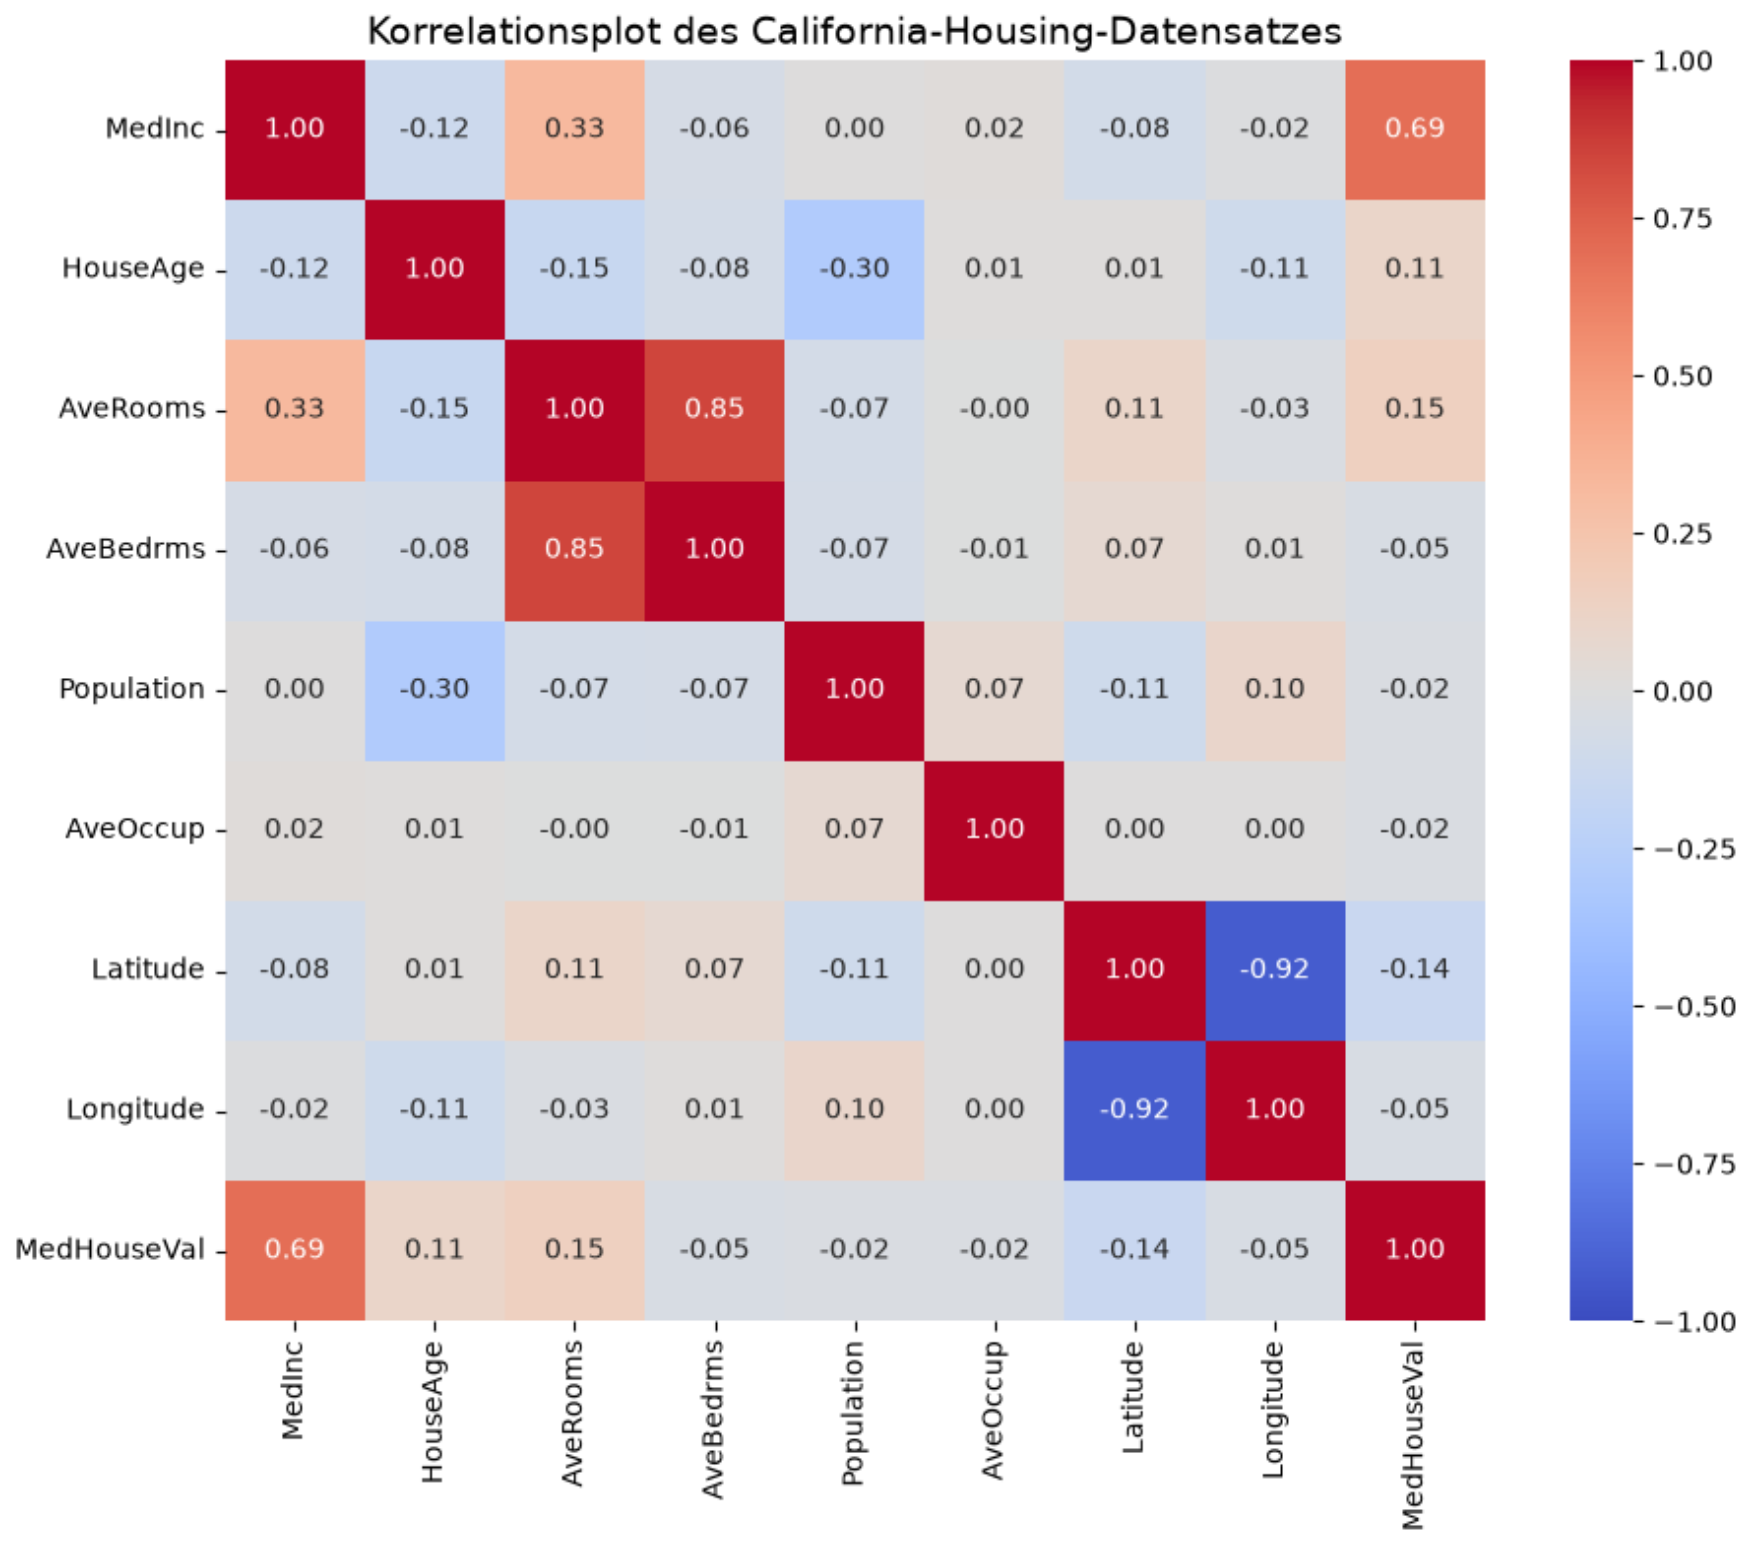
\includegraphics[width=0.9\textwidth]{./asset/image/Aufgabe2e.png}
    \caption{Korrelationsplot des California-Housing-Datensatzes (\textit{Quelle: Eigene Darstellung})}
    \label{fig:aufgabe2e}
\end{figure}

Die Korrelationen der unabhängigen Variablen mit der Zielvariable \texttt{MedHouseVal} sind:

\begin{verbatim}
Korrelationen mit der Zielvariable MedHouseVal:
MedHouseVal    1.000000
MedInc         0.688075
AveRooms       0.151948
HouseAge       0.105623
AveOccup      -0.023737
Population    -0.024650
Longitude     -0.045967
AveBedrms     -0.046701
Latitude      -0.144160
Name: MedHouseVal, dtype: float64

Die größte Korrelation mit MedHouseVal zeigt 'MedInc' mit einem Wert von 0.6881
\end{verbatim}

\subsection{Interpretation}

Die Korrelationsmatrix wird mit \texttt{df\_california.corr()} berechnet. Der Korrelationsplot mit \texttt{sns.heatmap()} visualisiert die paarweisen Korrelationen zwischen allen Variablen. Die Farbkodierung reicht von Blau (\textit{negative Korrelation}) über Weiß (\textit{keine Korrelation}) bis Rot (\textit{positive Korrelation}). Auf der Diagonalen sind die Korrelationen einer Variable mit sich selbst (\textit{Wert = 1,0}) dargestellt.

Die größte Korrelation mit der Zielvariable \texttt{MedHouseVal} zeigt die Variable \texttt{MedInc} mit einem Korrelationskoeffizienten von etwa 0.69. Dies bestätigt den im Pairplot (\textit{Aufgabe 2d}) bereits sichtbaren positiven linearen Zusammenhang zwischen dem mittleren Einkommen und dem mittleren Hauswert.

Die Variable \texttt{AveRooms} zeigt mit etwa 0.15 eine schwache positive Korrelation mit dem Hauswert. \texttt{Latitude} zeigt eine negative Korrelation von etwa -0.14, was darauf hindeutet, dass nördlichere Gebiete tendenziell niedrigere Hauswerte aufweisen. Die Variablen \texttt{AveOccup}, \texttt{Population} und \texttt{Longitude} zeigen nahezu keine Korrelation mit dem Hauswert.

\cleardoublepage

% ======================================= f =====================================

\section{Train-Test-Split und lineare Regression (f)}
\label{sec:2f}

\subsection{Aufgabenstellung}

Der Datensatz wird in Trainings- und Testdaten aufgeteilt. Es wird ein lineares Regressionsmodell ohne die Spalten \texttt{Latitude} und \texttt{Longitude} erstellt. Der Mean Squared Error (\textit{\acs{MSE}}) und der \acs{$R^2$-Score} werden berechnet.

\subsection{Lösung}

Zunächst werden die Spalten \texttt{Latitude} und \texttt{Longitude} aus den unabhängigen Variablen entfernt. Die Zielvariable ist \texttt{MedHouseVal}. Der Datensatz wird mit \texttt{train\_test\_split()} in Trainings- (\textit{80\%}) und Testdaten (\textit{20\%}) aufgeteilt. Das lineare Regressionsmodell wird mit \texttt{LinearRegression()} aus \texttt{sklearn.linear\_model} erstellt und mit den Trainingsdaten trainiert. Die Vorhersage erfolgt auf den Testdaten. Der Mean Squared Error wird mit \texttt{mean\_squared\_error()} und der \acs{$R^2$-Score} mit \texttt{r2\_score()} berechnet.

\lstinputlisting[
    language=Python, 
    caption={Train-Test-Split und lineare Regression}, 
    label={lst:aufgabe2f}
]{asset/code/Aufgabe2f.tex}

\subsection{Ausgabe}

Die Ausgabe zeigt den Mean Squared Error und den \acs{$R^2$-Score} des linearen Regressionsmodells:

\begin{verbatim}
Mean Squared Error (MSE): 0.6422
R2 Score: 0.5099
\end{verbatim}

\subsection{Interpretation}

Die Aufteilung in Trainings- und Testdaten erfolgt mit \texttt{train\_test\_split()} im Verhältnis 80:20. Der Parameter \texttt{random\_state=42} sorgt für Reproduzierbarkeit. Die Spalten \texttt{Latitude} und \texttt{Longitude} werden mit \texttt{drop()} aus den unabhängigen Variablen entfernt, da sie in dieser Teilaufgabe nicht verwendet werden sollen.

Das lineare Regressionsmodell wird mit \texttt{LinearRegression().fit(\textit{X\_train}, \textit{y\_train})} trainiert. Der Mean Squared Error von etwa 0.6422 bedeutet, dass die quadrierten Vorhersagefehler im Durchschnitt etwa 0.6422 betragen. Der \acs{$R^2$-Score} von etwa 0.5099 bedeutet, dass das Modell etwa 51\% der Varianz der Zielvariable erklärt. Dies ist ein akzeptabler Wert für ein lineares Modell, zeigt aber, dass nichtlineare Zusammenhänge (\textit{\acs{z. B.} durch \texttt{Latitude} und \texttt{Longitude}}) nicht erfasst werden.

\subsection{Bemerkung zur Reproduzierbarkeit}

Der Parameter \texttt{random\_state=42} wird verwendet, um die zufällige Aufteilung reproduzierbar zu machen. Dadurch erhält jeder Lauf des Codes das gleiche Ergebnis.

\cleardoublepage

% ======================================= g =====================================

\section{Entscheidungsbaum-Regression (g)}
\label{sec:2g}

\subsection{Aufgabenstellung}

Es wird ein Regressionsmodell mit einem Entscheidungsbaum erstellt (\textit{wieder ohne die Spalten \texttt{Latitude} und \texttt{Longitude}}). Es wird ermittelt, ab welcher maximalen Tiefe (\textit{\texttt{max\_depth}}) dieses Modell bessere Resultate liefert als die lineare Regression aus Aufgabe 2 f.

\subsection{Lösung}

Es wird eine Schleife über verschiedene maximale Tiefen von 1 bis 20 durchgeführt. Für jede Tiefe wird ein Entscheidungsbaum-Regressionsmodell mit \texttt{DecisionTreeRegressor()} aus \texttt{sklearn.tree} erstellt, mit den Trainingsdaten trainiert und auf den Testdaten evaluiert. Die \acs{$R^2$-Score} werden gespeichert und mit dem \acs{$R^2$-Score} der linearen Regression (\textit{0.5099}) verglichen. Die erste Tiefe, bei der der \acs{$R^2$-Score} der Entscheidungsbaum-Regression den \acs{$R^2$-Score} der linearen Regression übersteigt, wird ermittelt.

\lstinputlisting[
    language=Python, 
    caption={Entscheidungsbaum-Regression mit verschiedenen Tiefen}, 
    label={lst:aufgabe2g}
]{asset/code/Aufgabe2g.tex}

\subsection{Ausgabe}

Die Ausgabe zeigt die \acs{$R^2$-Score} für verschiedene maximale Tiefen sowie die Tiefe, ab der der Entscheidungsbaum besser ist als die lineare Regression:

\begin{verbatim}
max_depth= 1  R2 Score: 0.2795
max_depth= 2  R2 Score: 0.4244
max_depth= 3  R2 Score: 0.5098
max_depth= 4  R2 Score: 0.5542
max_depth= 5  R2 Score: 0.5938
max_depth= 6  R2 Score: 0.6135
max_depth= 7  R2 Score: 0.6293
max_depth= 8  R2 Score: 0.6326
max_depth= 9  R2 Score: 0.6078
max_depth=10  R2 Score: 0.5911
max_depth=11  R2 Score: 0.5717
max_depth=12  R2 Score: 0.5546
max_depth=13  R2 Score: 0.5267
max_depth=14  R2 Score: 0.4959
max_depth=15  R2 Score: 0.4664
max_depth=16  R2 Score: 0.4459
max_depth=17  R2 Score: 0.4363
max_depth=18  R2 Score: 0.4183
max_depth=19  R2 Score: 0.4176
max_depth=20  R2 Score: 0.4097

Die lineare Regression hat einen R2 Score von 0.5099
Der Entscheidungsbaum ist ab einer Tiefe von 4 besser als die lineare Regression.
\end{verbatim}

\begin{figure}[h]
    \centering
    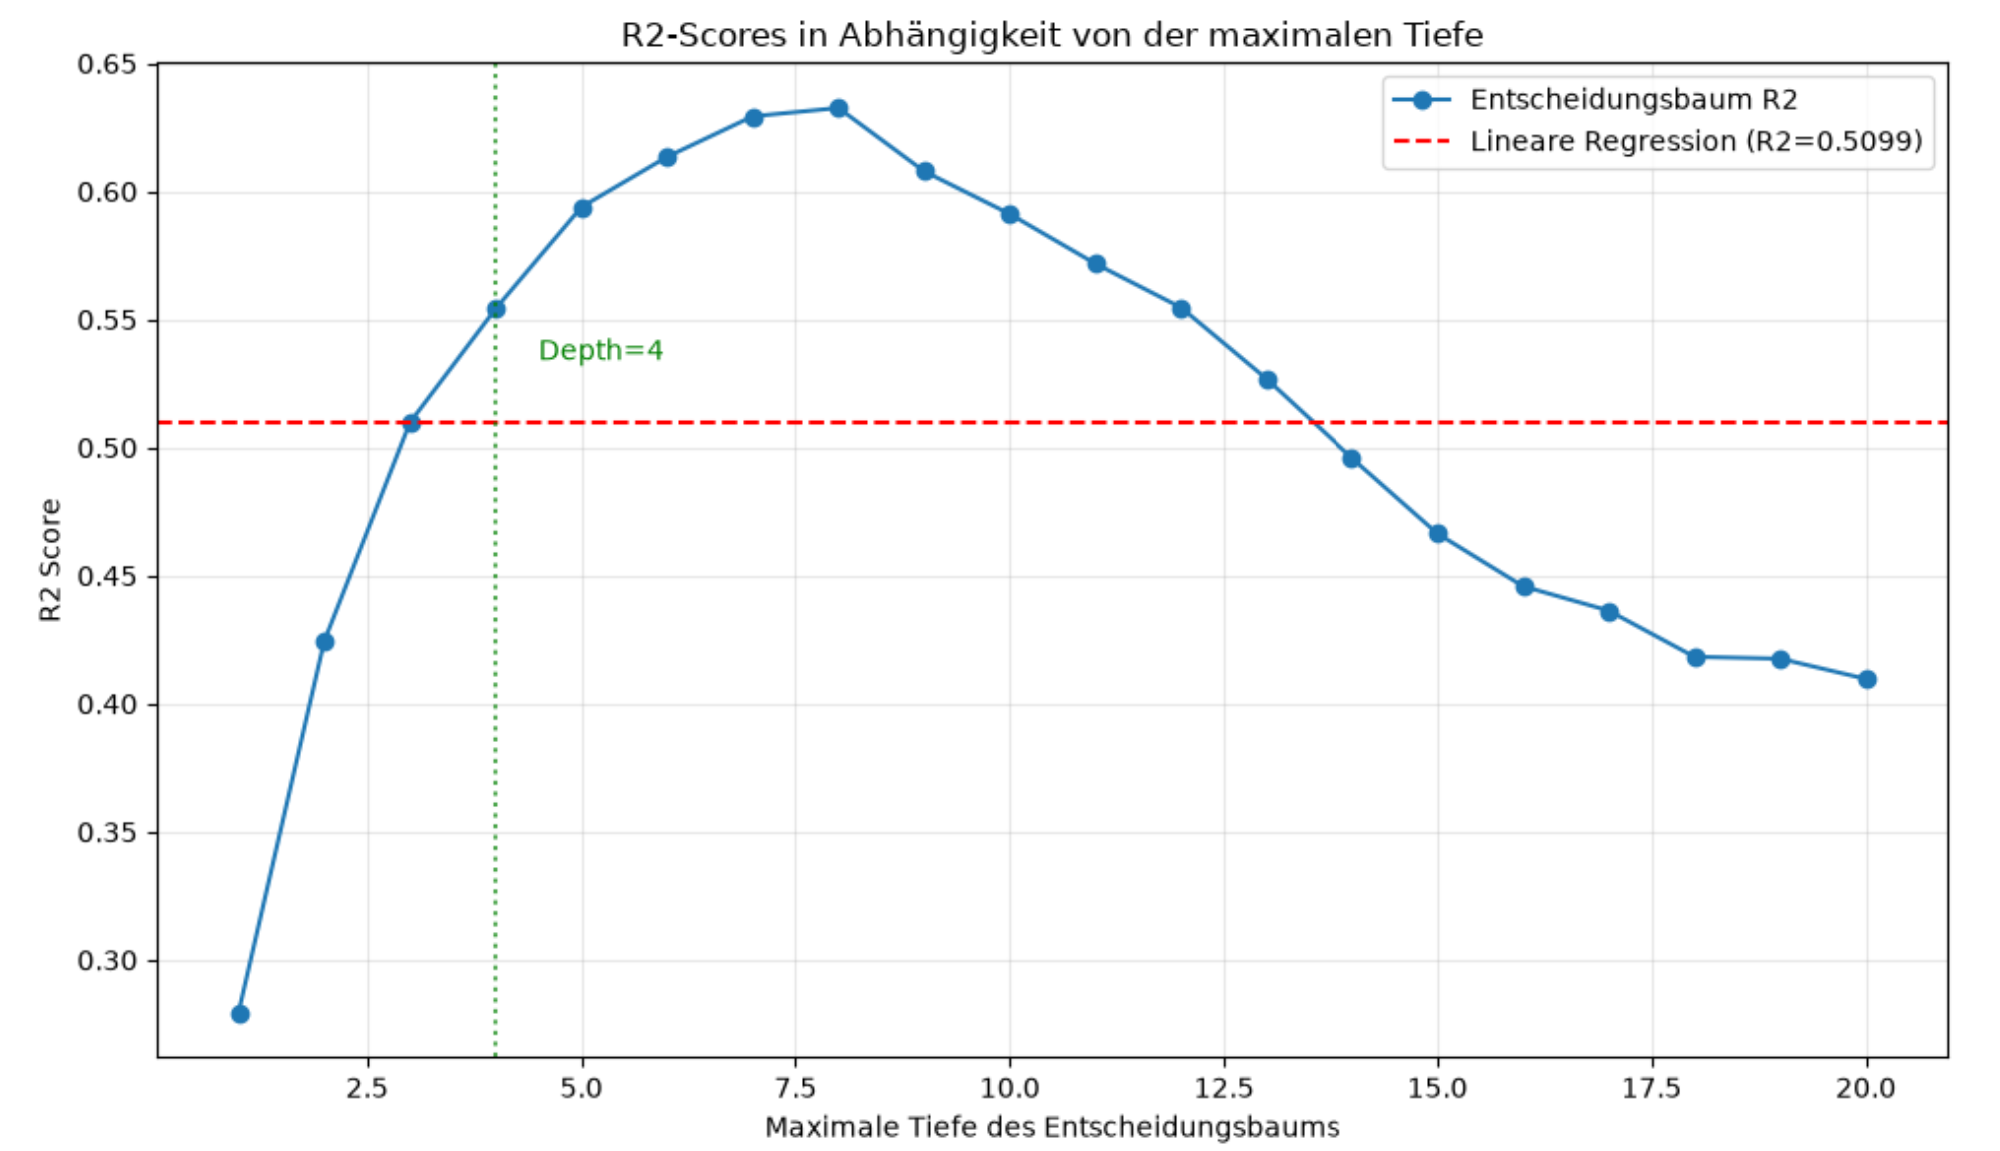
\includegraphics[width=0.9\textwidth]{./asset/image/Aufgabe2g.png}
    \caption{\acs{$R^2$-Score}s in Abhängigkeit von der maximalen Tiefe des Entscheidungsbaums (\textit{Quelle: Eigene Darstellung})}
    \label{fig:aufgabe2g}
\end{figure}

\subsection{Interpretation}

Die Entscheidungsbaum-Regression wird mit \texttt{DecisionTreeRegressor(\textit{random\_state=42})} für verschiedene maximale Tiefen trainiert. Der Parameter \texttt{random\_state=42} sorgt für Reproduzierbarkeit. Für jede Tiefe wird der \acs{$R^2$-Score} auf den Testdaten berechnet und gespeichert.

Der \acs{$R^2$-Score} der linearen Regression aus Aufgabe 2f beträgt 0.5099. Die Entscheidungsbaum-Regression erreicht bereits bei geringen Tiefen Werte nahe dem linearen Modell. Ab einer Tiefe von 4 übersteigt der \acs{$R^2$-Score} des Entscheidungsbaums den der linearen Regression. Die besten Ergebnisse werden im Bereich von Tiefe 7 bis 8 erzielt, wo der \acs{$R^2$-Score} auf etwa 0.63 ansteigt. Dies zeigt, dass der Entscheidungsbaum nichtlineare Zusammenhänge besser erfassen kann als das lineare Modell.

Bei sehr großen Tiefen (\textit{ab etwa 14}) sinkt der \acs{$R^2$-Score} wieder unter den Wert der linearen Regression, was auf Overfitting hindeutet: Der Entscheidungsbaum lernt die Trainingsdaten zu gut und verliert seine Generalisierungsfähigkeit.

\cleardoublepage

% ======================================= h =====================================

\section{Verfälschung durch Weglassen von Latitude und Longitude (h)}
\label{sec:2h}

\subsection{Aufgabenstellung}

Es wird analysiert, auf welche Weise die Ergebnisse der Regression verfälscht werden, wenn die Spalten \texttt{Latitude} und \texttt{Longitude} weggelassen werden. Es wird beschrieben, wie grundsätzlich verfahren werden kann, um diese beiden Spalten in der Regression zu berücksichtigen.

\subsection{Verfälschung der Ergebnisse durch Weglassen}

Die Spalten \texttt{Latitude} und \texttt{Longitude} enthalten geografische Informationen, die räumliche Strukturen im Datensatz abbilden. Werden diese weggelassen, gehen diese räumlichen Informationen verloren.

Die Verfälschung der Ergebnisse äußert sich wie folgt:

\begin{itemize}
    \item \textbf{Räumliche Abhängigkeiten werden ignoriert:} Hauswerte weisen oft räumliche Cluster auf, benachbarte Gebiete haben ähnliche Hauswerte. Durch Weglassen von \texttt{Latitude} und \texttt{Longitude} wird diese räumliche Autokorrelation nicht berücksichtigt.
    \item \textbf{Verzerrung der Koeffizienten:} Andere Variablen (\textit{\acs{z. B.} \texttt{MedInc}}) können fälschlicherweise einen zu großen Einfluss erhalten, weil sie teilweise die räumlichen Effekte "kompensieren" müssen.
    \item \textbf{Unterschätzung der Modellgüte:} Räumliche Muster, die nicht durch andere Variablen erklärt werden, bleiben unberücksichtigt, was zu einer geringeren Vorhersagegenauigkeit führt.
    \item \textbf{Verlust von Kontextinformationen:} Die geografische Lage ist ein wichtiger Prädiktor für Hauswerte (\textit{\acs{z. B.} Nähe zum Meer}, \textit{Stadtzentrum}). Ohne diese Information geht wertvolles Wissen verloren.
\end{itemize}

\subsection{Möglichkeiten zur Berücksichtigung von Latitude und Longitude}

Um die beiden Spalten \texttt{Latitude} und \texttt{Longitude} in der Regression zu berücksichtigen, können grundsätzlich folgende Verfahren angewendet werden:

\begin{enumerate}
    \item \textbf{Direkte Integration als numerische Features:} \texttt{Latitude} und \texttt{Longitude} werden als zusätzliche numerische Features in das Modell aufgenommen. Dies ist die einfachste Methode und erfasst lineare räumliche Effekte.
    \item \textbf{Polynomiale Features:} Mit \lstinline{PolynomialFeatures} aus \lstinline{sklearn.preprocessing} können nichtlineare räumliche Effekte modelliert werden, \textit{\acs{z. B.}} durch Hinzufügen von quadratischen Termen (\textit{\lstinline{Latitude**2}, \lstinline{Longitude**2}}) oder Interaktionstermen (\textit{\lstinline{Latitude * Longitude}}).
    \item \textbf{Räumliche Features extrahieren:} Aus den Koordinaten können neue Features abgeleitet werden, \textit{\acs{z. B.}}:
    \begin{itemize}
        \item Distanz zu bestimmten Punkten (\textit{Stadtzentrum}, \textit{Küste}, \textit{Arbeitszentren})
        \item Nachbarschaftsindikatoren (\textit{\acs{z. B.} Mittelwert der Hauswerte benachbarter Gebiete})
        \item Räumliche Cluster-Labels (\textit{\acs{z. B.} mittels K-Means-Clustering auf den Koordinaten})
    \end{itemize}
    \item \textbf{Räumliche Regressionsmodelle:} Es werden spezielle räumliche Regressionsmodelle verwendet, die räumliche Abhängigkeiten explizit modellieren, wie \textit{\acs{z. B.}}:
    \begin{itemize}
        \item \textbf{Spatial Autoregressive Models (\textit{\acs{SAR}}):} Modellieren die räumliche Abhängigkeit der Zielvariable.
        \item \textbf{Spatial Error Models (\textit{\acs{SEM}}):} Modellieren die räumliche Abhängigkeit in den Fehlertermen.
    \end{itemize}
    \item \textbf{Interaktionsterme:} Es werden Interaktionen zwischen \texttt{Latitude}, \texttt{Longitude} und anderen Variablen erstellt (\textit{\acs{z. B.}} $\texttt{MedInc} \times \texttt{Latitude}$), um regionale Unterschiede im Einfluss anderer Variablen zu erfassen.
\end{enumerate}

\subsection{Ausgabe}

Die folgende Visualisierung zeigt die räumliche Verteilung der Hauswerte in Kalifornien:

\begin{figure}[h]
    \centering
    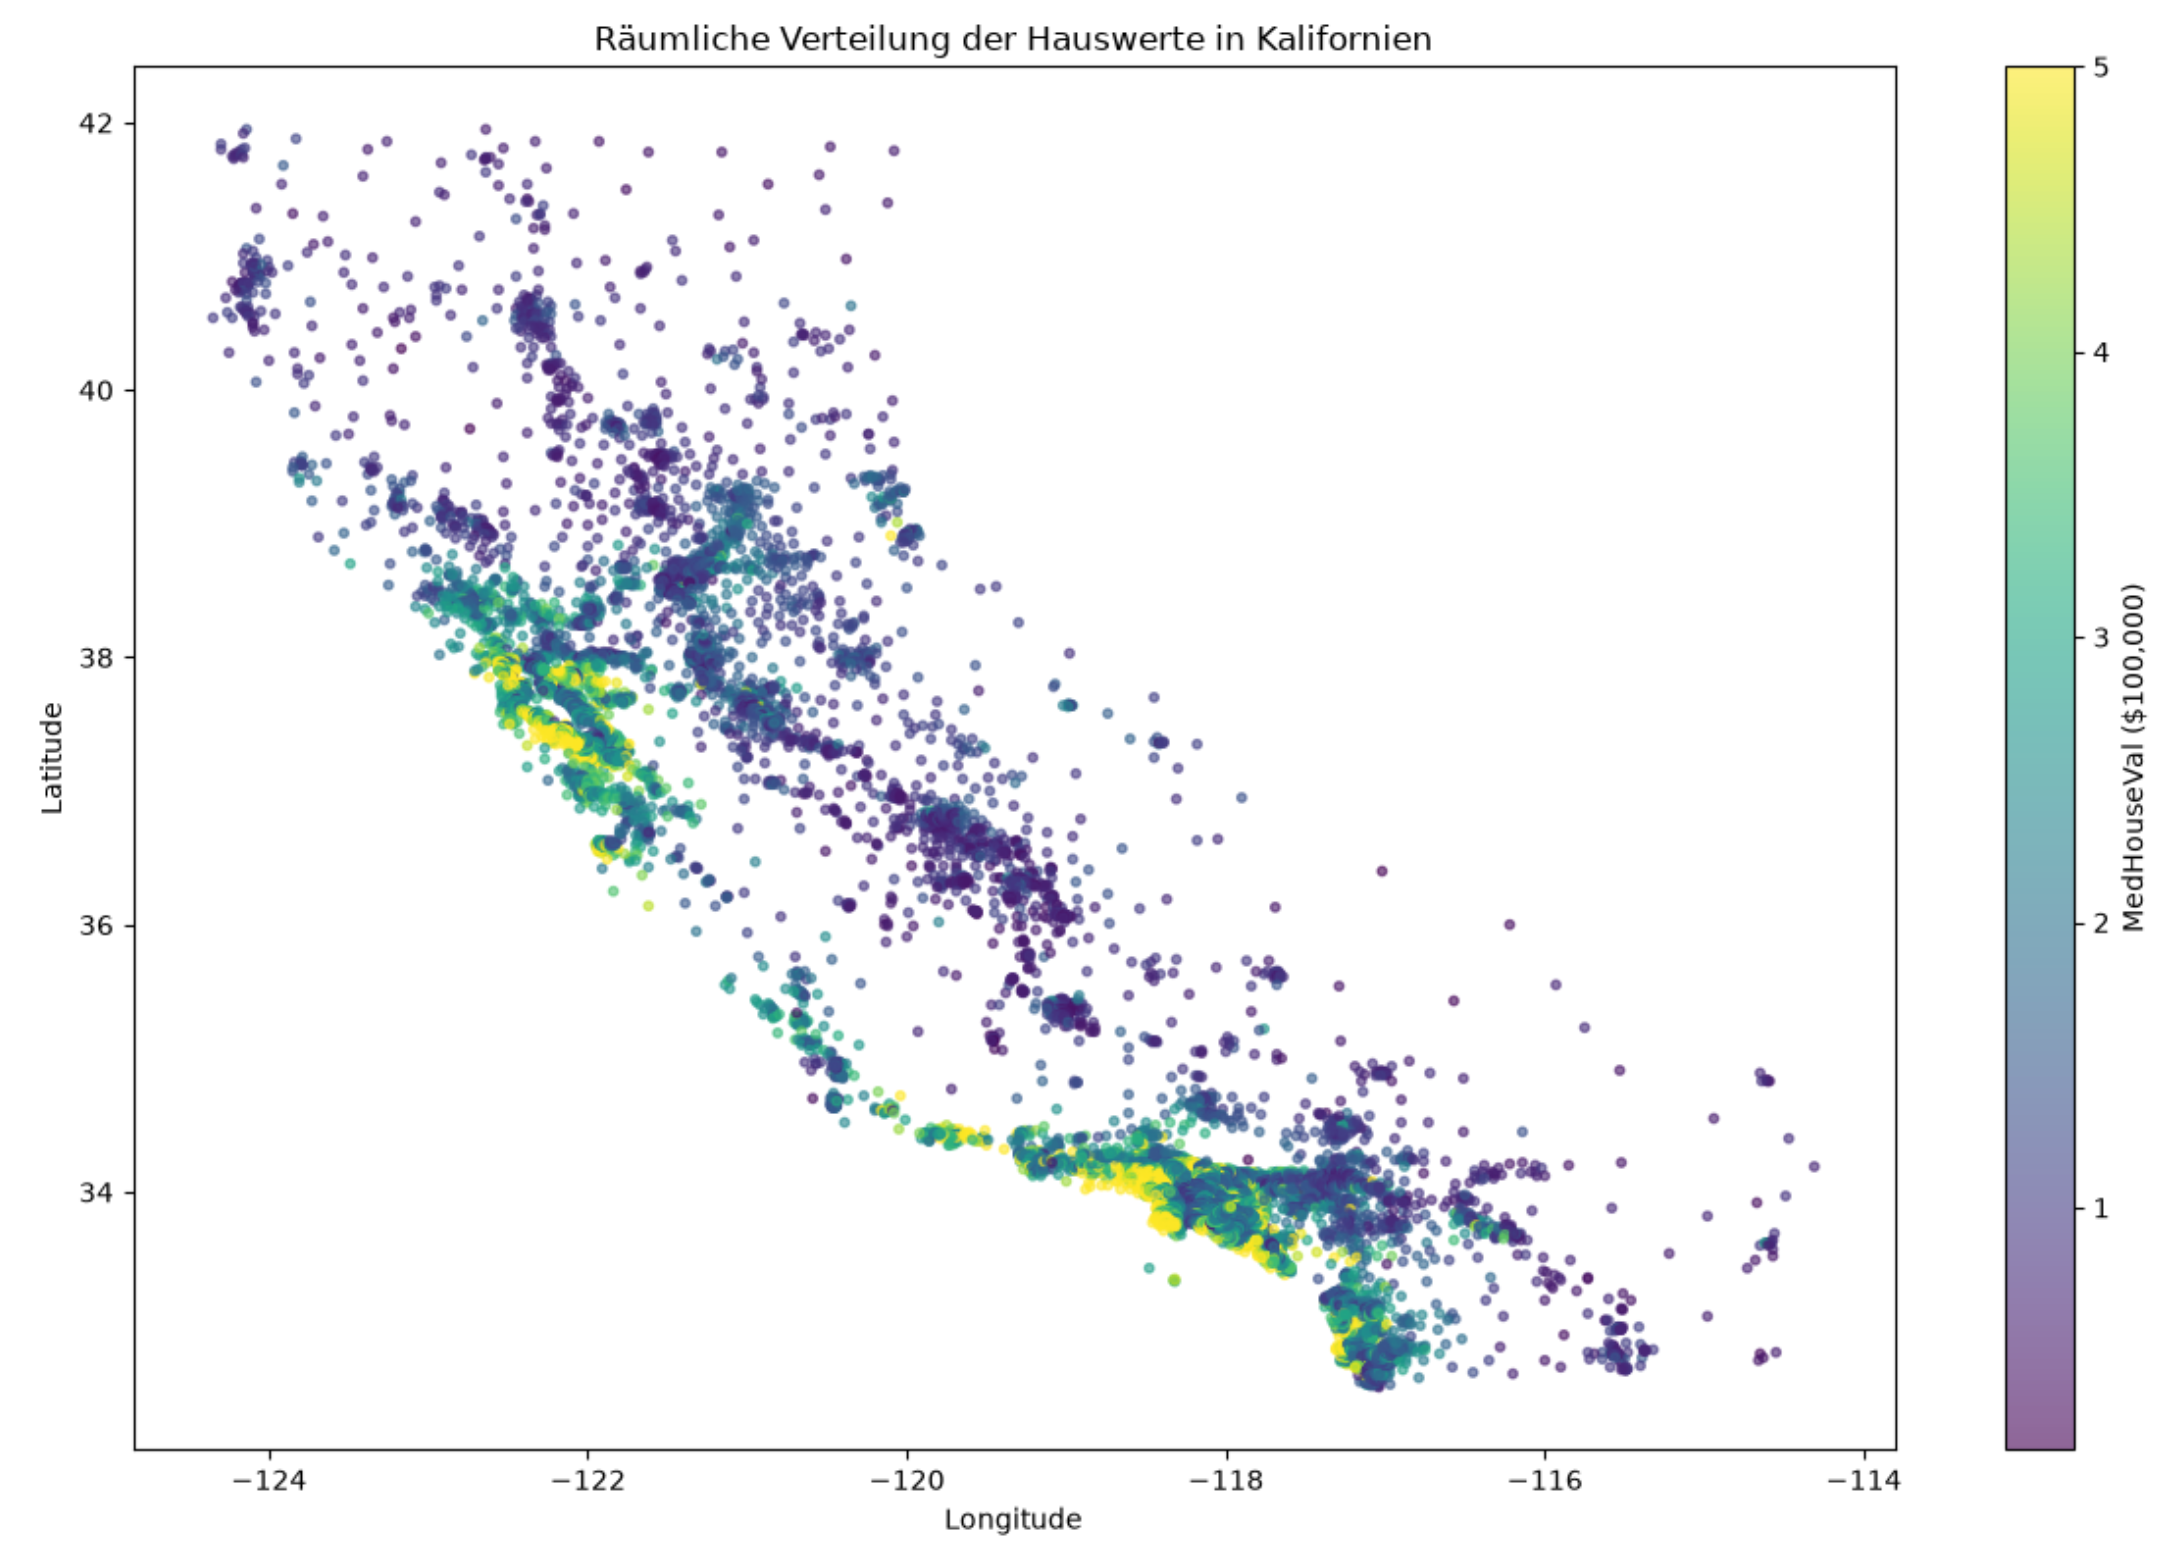
\includegraphics[width=0.9\textwidth]{./asset/image/Aufgabe2h.png}
    \caption{Räumliche Verteilung der Hauswerte in Kalifornien (\textit{Quelle: Eigene Darstellung})}
    \label{fig:aufgabe2h}
\end{figure}

Der Scatter-Plot wurde mit folgendem Code erstellt:

\lstinputlisting[
    language=Python,
    caption={Visualisierung der räumlichen Verteilung der Hauswerte},
    label={lst:aufgabe2h}
]{asset/code/Aufgabe2h.tex}

\subsection{Interpretation}

Das Weglassen von \texttt{Latitude} und \texttt{Longitude} führt zu einer Verfälschung der Regressionsergebnisse, da räumliche Abhängigkeiten nicht berücksichtigt werden. Hauswerte sind in Kalifornien stark von der geografischen Lage abhängig- Küstennähe, Nähe zu Ballungszentren und regionale Wirtschaftskraft spielen eine entscheidende Rolle. Ohne diese Informationen kann das Modell diese Effekte nicht erfassen.

Die einfachste und praktikabelste Methode zur Berücksichtigung ist die direkte Aufnahme von \texttt{Latitude} und \texttt{Longitude} als numerische Features. Für eine verbesserte Modellierung können Polynome oder Interaktionsterme hinzugefügt werden. Für komplexere räumliche Strukturen bieten sich räumliche Regressionsmodelle oder die Extraktion von räumlichen Clustern an.

In der Praxis hat sich gezeigt, dass die Berücksichtigung geografischer Informationen die Modellgüte deutlich verbessern kann, da sie sowohl direkte als auch indirekte (\textit{über andere Variablen vermittelte}) räumliche Effekte erfasst.

% ==============================================================================
% =============================== Ende Aufgabe 2 ===============================
% ==============================================================================